\chapter{Privacy and Data Protection}
\thispagestyle{chapterInit}

\section{\textit{On Privacy}}
    \subsection{Definizioni}
        Informalmente possiamo definire la privacy con il principio di auto-determinazione, ovvero ognuno ha il diritto di controllare le informazioni che lo riguardano.\newline
        Questo principio implica diversi possibilità di gestire le nostre informazioni:
        \begin{itemize}
            \item Chi ha diritto a vedere cosa (Riguarda \texttt{AC})
            \item Chi ha diritto a usare cosa (Riguarda \texttt{UC})
            \item Per che cosa possono usarlo (Riguarda \texttt{PC})
            \item A chi possono trasferirlo (Riguarda \texttt{DTC})
            \item \dots
        \end{itemize}
        Garantire tutti queste possibilità di controllo è molto difficile in quando correlare i dati e/o azioni è molto complesso. Questo però significa che esiste ancora qualche possibilità di mantenere l'anonimato anche se può essere molto difficile.
        \paragraph{\textit{Security} vs \textit{Privacy}}
        La \textit{security} e la \textit{privacy} sono due concetti che possono apparentemente sembrare simili ma che in realtà condividono solo una piccola porzione di concetti in comune. Infatti queste hanno in comune lo scopo di proteggere le informazioni personali, ma la \textit{security} si occupa anche della triade \texttt{CIA}\footnote{Confidentiality, Integrity, Availability, vedi \ref{sec:ciaTriad} - \nameref{sec:ciaTriad}} mentre la \textit{privacy} si occupa inoltre dell'uso e visualizzazione delle informazioni in maniera corretta, della raccolta e qualità dei dati e informazioni personali e della loro gestione.
    \subsection{L'acronimo \texttt{LINDDUN}}
        L'acronimo \texttt{LINDDUN} sta per:
        \begin{itemize}
            \item \textbf{Linkability}
            \item \textbf{Identifiability}
            \item \textbf{Non-repudiation}
            \item \textbf{Detectability}
            \item \textbf{Disclosure of information}
            \item \textbf{Unawareness}
            \item \textbf{Non-compliance}
        \end{itemize}
        Questo acronimo è stato creato per definire i principi fondamentali della privacy e della protezione dei dati.
        \subsubsection{Linkability}
            La \textit{linkability} è la capacità di distinguere se due o più \textbf{elementi di interesse} (\textit{Items of Interest} - \texttt{IoI}) sono correlati o meno tra loro senza conoscere l'identità del soggetto al quale sono associati. Esempio di questo può essere: la cronologia di navigazione di uno stesso utente, le entry su tabelle diverse collegate ad uno stesso utente, \dots\newline
            Come conseguenza sussiste la possibilità che venga compromessa l'identità (e il principio di \textit{identifiability}) quando troppe informazioni sono collegate tra loro. Inoltre c'è il rischio di inferenza (o \textit{inference}), questo nel caso nel quale un gruppo di informazioni è associabile, il che può comportare a discriminazioni o \textit{targeting} verso (ad esempio) un particolare gruppo di persone che vive in una determinata zona.
        \subsubsection{Identifiability}
            L'\textit{identifiability} è la capacità di identificare un particolare soggetto tra un gruppo di soggetti anonimi, questo se non si riesce a nascondere il collegamento tra l'identità di un soggetto ed un \texttt{IoI}. Ad esempio: riuscire ad identificare chi è il lettore di una pagina web, oppure a chi si riferiscono i dati di una tabella. Conseguenza della mancata protezione del principio di \textit{identifiability} è la presenza di gravi violazioni della \textit{privacy}.
        \subsubsection{Non-repudiation}
            La \textit{non-repudiation} è la capacità di garantire che un soggetto non possa negare di aver compiuto una determinata azione. Questo principio è molto importante in ambito legale, in quanto se un soggetto non può negare di aver compiuto una determinata azione, allora è possibile dimostrare che ha compiuto un'azione illecita. Questo principio è molto importante in ambito di \textit{e-commerce} e \textit{e-government} ovvero nel caso di votazioni \textit{on-line} o di contratti stipulati \textit{on-line}. Come conseguenza se viene violato un \textit{dataset} con all'interno delle prove che un soggetto è un informatore di un'organizzazione, allora questo può comportare gravi conseguenze per la persona coinvolta.
        \subsubsection{Detectability}
            La \textit{detectability} è la capacità di distinguere se una \texttt{IoI} esiste o meno. Questo determina che un attaccante conosce o meno se l'informazione è contenuta in un determinato \textit{dataset}. Questo principio è molto importante in ambito di \textit{data mining} è possibile infatti dedurre certe informazioni senza avere accesso ad esse.
        \subsubsection{Disclosure of information}
            Ovvero la perdita di \textit{confidentiality}. Vedi \ref{sec:ciaTriad} - \nameref{sec:ciaTriad}.
        \subsubsection{Unawareness}
            La \textit{unawareness} è la mancata consapevolezza degli effetti della condivisione di una informazione. Questo principio è molto importante in ambito di \textit{social network} in quanto spesso non si è consapevoli delle conseguenze della condivisione di determinate informazioni quali ad esempio carte fedeltà, servizi online, \dots\newline
            Idealmente ogni utente deve essere consapevole degli effetti della condivisione di tali informazioni verso terzi. Più informazioni sono disponibili più queste sono associabili.
        \subsubsection{Non-compliance}
            La \textit{non-compliance} è la mancata osservanza delle regole di protezione della privacy. Questo porta a multe e/o perdita di credibilità per l'organizzazione che non rispetta le regole di protezione della privacy.
        
        \begin{figure}[H]
            \centering
            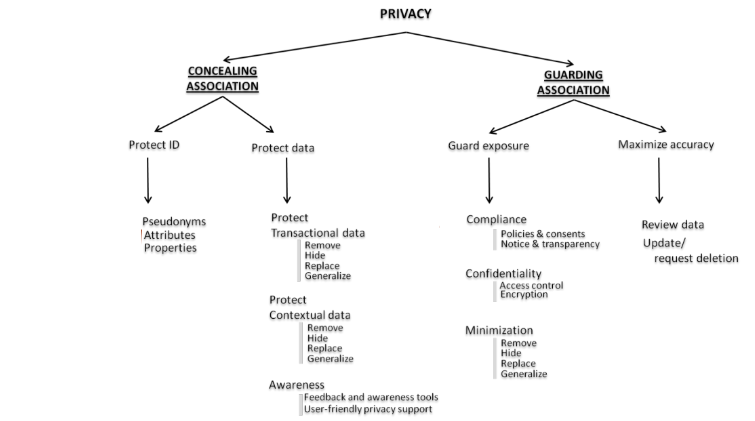
\includegraphics[width=0.6\textwidth]{09/LINDDUN-mitigazioni.png}
            \caption{Mitigazioni per i principi di \texttt{LINDDUN}}
        \end{figure}
\section{On Anonymization}
    \subsection{Anonimizzazione e attacchi basati su \textit{linkability}} 
        \subsubsection{Anonimizzazione dei dati}
            L'anonimizzazione è definita come il processo di rimozione delle \texttt{PII} - \textit{Personally Identifying Information} come ad esempio: nome, cognome, indirizzo, \dots\newline
            Il problema sussiste che a lato pratico/tecnico \texttt{PII} non ha una definizione precisa. È definito invece cosa fare quando è persa l'anonimato di quella informazione: contattare l'utente, notificare l'incidente, \dots\newline
            Nell'avvento di un \textit{data-leak} qualsiasi tipo di informazione può essere considerata \texttt{PII}.\footnote{Vedi Netflix \textit{data-leak} del 2006. \href{https://www.cs.utexas.edu/~shmat/netflix-faq.html}{Studio del \textit{data-leak} di Netflix - Università del Texas}}
        \subsubsection{Attacchi basati su \textit{linkability}}
            Gli attacchi basati su \textit{linkability} sono attacchi che sfruttano la correlazione tra due o più \texttt{IoI} anche presi da dataset diversi. Questo tipo di attacchi sono molto pericolosi in quanto possono compromettere la privacy di un utente. Alcune volte inoltre per legge è richiesto che vengano pubblicati i dati in forma anonima, spesso incrociando questi dati con altri dataset è possibile risalire a delle informazioni riguardanti questa persona, e nel caso peggiore risalire all'identità di questa persona.\newline
            Ciò accade in quanto spesso nei \textit{dataset} resi pubblici gli attributi demografici quali ad esempio: età, sesso, \texttt{CAP}, \dots sono presenti e possono essere utilizzati per incrociare i dati e risalire all'identità di una persona. Gli attributi quali data di nascita, sesso, \texttt{CAP} sono chiamati \textit{Quasi-identifiers} e anche se non sono direttamente identificativi, possono essere utilizzati per scoprire ulteriori informazioni su quella persona e eventualmente risalirne all'identità. Pubblicare un \textit{dataset} anonimo con dei \textit{Quasi-identifiers} è molto pericoloso e spesso è equivalente a pubblicare un \textit{dataset} non anonimo. Dati sensibili non dovrebbero \textbf{mai} essere pubblicati con dei \textit{Quasi-identifiers}, ne tanto meno con attributi chiave.
        \subsubsection{Mitigazione attacchi \textit{linkability} - $k$-anonymity}
                Pubblicare un dataset $k$-anonimo significa che ogni persona non può essere distinta da almeno $k-1$ altri individui diversi. Quindi ogni insieme di \textit{Quasi-identifier} appare almeno $k$ volte all'interno di uno stesso \textit{dataset}. 
            \paragraph{Come ottenere $k$-anonimità}
                Per ottenere $k$-anonimità si può agire in due modi distinti: \textbf{generalizzazione} e \textbf{soppressione} degli attributi.
                \subparagraph{Generalizzazione} La generalizzazione consiste nel sostituire un attributo con un suo super-insieme (es: Se l'età è 25, generalizzarla a 20-30 o 2*).
                \subparagraph{Soppressoione} La soppressione consiste nel rimuovere un attributo dal dataset. Queste due tecniche possono essere utilizzate insieme per ottenere $k$-anonimità.
    \subsection{Pseudo-anonimizzazione}
        La pseudo-anonimizzazione è una tecnica che consiste nel sostituire i dati identificativi con altri. Questo però può tenere traccia dell'identità originale di una persona e sussiste il rischio che un soggetto venga identificato tramite attacchi di \textit{re-identification}, come gli attacchi basati su \textit{linkability}. In certe situazioni gli pseudonimi possono contenere loro stessi delle informazioni sulla persona, quali ad esempio: l'anno di nascita è contenuto nel codice fiscale. Da questo punto di vista è importante che gli pseudonimi siano generati in modo che questi siano resilienti a \textit{data-loss} e \textit{data-leak}.
        \subsubsection{Definizione di fuzioni di pseudonimizzazione}
            Una ``Funzione di pseudonimizzazione'' è una funzione che ``mappa'' un dato identificativo in uno pseudonimo. Questa funzione ha come requisito che se $d1$ e $d2$ sono due dati distinti, allora $f(d1)=pseudo1 \neq pseudo2=f(d2)$. Questo in quanto la funzione che ritorna il dato identificativo (funzione inversa) deve essere in grado di ritornare il dato originale senza ambiguità. Questo non esclude che uno stesso dato non possa essere associato a più pseudonimi. In ogni caso esistono delle informazioni che servono ad associare uno pseudonimo ad un dato, le quali vengono chiamate \textbf{\textit{pseudonymisation secret}} e devono essere protette in modo che non possano essere associate ad un dato. La forma più semplice di \textit{pseudonymisation secret} è una tabella di ``mapping'' tra dati e pseudonimi.
        \subsubsection{Inplementazione di funzioni di pseudonimizzazione} 
            Le funzioni di pseudonimizzazione possono essere implementate in diversi modi, tra i quali:
            \begin{description}
                \item[Counter] Gli identificatori sono sostituiti con un numero, il quale viene incrementato ogni volta che viene generato uno pseudonimo. Questo metodo è molto semplice ma non è sicuro. La non-sicurezza di questo metodo è data dalla poca scalabilità per grandi \texttt{DB} e dal fatto che l'ordine può dare informazioni sull'ordine delle informazioni.
                \item[Generatore di numeri casuali] Gli identificatori sono sostituiti con numeri casuali. Questo metodo è più sicuro del precedente ma è difficile da implementare evitando ripetizioni senza memorizzare i numeri generati.
                \item[Funzioni di \textit{Hash}] Il \textit{digest} dell'identificativo è lo pseudonimo generato. Questo metodo è considerato inadeguato in quanto non è reversibile ed è soggetto ad attacchi di \textit{brute force} e \textit{dictionary attack}.
                \item[Encryption] L'identificativo è cifrato tramite cifrari a blocchi come \texttt{AES} o \texttt{DES}. In questo metodo la chiave usata per cifrare i dati è usata sia come \textit{pseudonymisation secret} che come \textit{recovery secret}. Viene usato il meccanismo di \textit{padding} in quanto gli identificativi spesso sono più piccoli della dimensione del blocco.
            \end{description} 
\section{\texttt{GDPR} - \textit{General Data Protection Regulation}}
    \subsection{In generale}
        La \textit{privacy} dei dati in europa è regolamentata dal \texttt{GDPR} - \textit{General Data Protection Regulation}. Questo regolamento è entrato in vigore il 25 Maggio 2018, questo in modo che sia una unica legge europea a trattare in materia di protezione dei dati. Il \texttt{GDPR} include: \begin{itemize}
            \item \textit{Safeguarding} dei dati.
            \item Modalità e forme di ottenimento del consenso da parte dell'utente.
            \item Identificazione delle leggi applicabili all'organizzazione sulla base dei dati trattati.
            \item Formazione dei dipendenti sull'uso dei dati, sulla sicurezza e sulla privacy.
        \end{itemize}
        Il \texttt{GDPR} protegge tutti i cittadini europei non facendo distinzione sul dove l'organizzazione raccoglie e conserva i dati. Inoltre il \texttt{GDPR} prescrive che in caso di \textit{data leak} che l'autorità competenti e gli utenti siano informati entro 72 ore dal \textit{data leak}. Se non si rispettano le normative del \texttt{GDPR} si rischiano multe fino al 4\% del fatturato annuo dell'organizzazione o fino a 20 milioni di euro.
    \subsection{Articoli selezionati}
        Nota dell'autore: \begin{quote}``Mi sono permesso di tradurre liberamente gli articoli selezionati e di riportare solo una parte di essi la quale ritengo essere la più importante per la comprensione del \texttt{GDPR} in funzione dello svolgimento del corso (e del superamento dell'esame). Tuttavia ciò non significa che il presente materiale sia completo e/o sufficiente a tali fini.''\end{quote}
        \subsubsection{Articolo 4: Definizioni}
            Questo articolo definisce le definizioni principali del \texttt{GDPR} quali:
            \begin{description}
                \item[\textit{Personal Data}] Qualsiasi informazione che identifica o può identificare una persona fisica direttamente o indirettamente.
                \item[\textit{Processing}] Qualsiasi operazione o insieme di operazioni effettuate su un dato personale o insieme di dati personali, sia che questo sia effettuato in modo automatizzato o meno, questo include: raccolta, consultazione, uso, divulgazione, \dots
                \item[\textit{Pseudonymisation}] Qualsiasi operazione sui dati personali in modo che tale dato non può più essere attribuito ad una persona senza l'uso di informazioni aggiuntive.
                \item[\textit{Controller}] La persona fisica o giuridica, l'autorità pubblica, l'agenzia o qualsiasi altro organismo che determina le finalità e i mezzi del trattamento dei dati personali. (In italia: \textit{Responsabile del trattamento})
                \item[\textit{Processor}] La persona fisica o giuridica, l'autorità pubblica, l'agenzia o qualsiasi altro organismo che tratta i dati personali per conto del \textit{controller}.
                \item[\textit{Consento}] Qualsiasi manifestazione di volontà libera, specifica, informata e inequivocabile della persona interessata con la quale questa accetta, mediante una dichiarazione o un'azione positiva, che i dati personali che la riguardano siano trattati.
                \item[\textit{Personal Data Breach}] Una violazione della sicurezza che comporta la distruzione, la perdita, l'alterazione, la divulgazione non autorizzata di dati personali trasmessi, conservati o altrimenti trattati.
            \end{description}
        \subsubsection{Articolo 7 - Condizioni per il consenso}
            \begin{enumerate}
                \item Dove il trattamento si basa sul consenso, il controller deve essere in grado di dimostrare che la persona interessata ha acconsentito al trattamento dei suoi dati personali.
                \item $\left[ \dots \right]$ le richieste per il consenso devono essere presentate in maniera tale che questa sia chiaramente distinguibile da altre questioni, in un modo intelligibile e di facile accesso, usando un linguaggio chiaro e semplice. Qualsiasi parte del consenso che non sia chiara o comprensibile non è valida.
                \item Il soggetto dei dati deve avere il diritto di ritirare il consenso in qualsiasi momento. $\left[ \dots \right]$ Il ritiro del consenso deve essere semplice quanto l'ottenimento di tale.
            \end{enumerate}
        \subsubsection{Articolo 32 - Sicurezza del trattamento}
            \begin{enumerate}
                \item Tenendo conto dello \textbf{stato dell'arte}\footnote{Per chi non lo sapesse (trai quali io stesso prima di ricercarlo), lo \textit{stato dell'arte} è il livello di conoscenza e di tecnologia raggiunto in un determinato campo di ricerca scientifica o tecnologica. In questo caso si riferisce allo stato della tecnologia informatica e della sicurezza informatica.} e \textbf{dei costi di implementazione}, nonché della natura, dell'ambito, del contesto e delle finalità del trattamento, nonché dei rischi, di varia probabilità e gravità, \textbf{per i diritti e le libertà delle persone fisiche}, il \textit{controller} e il \textit{processor} devono attuare misure \textit{tecniche e organizzative adeguate per garantire un livello di sicurezza adeguato al rischio}, compreso, tra l'altro, 
                    \begin{enumerate}
                        \item la \textbf{pseudonimizzazione} e la \textbf{cifratura} dei dati personali;
                        \item la capacità di garantire la \textbf{riservatezza}, \textbf{l'integrità}, \textbf{la disponibilità} e la \textbf{resilienza} dei sistemi e dei servizi di trattamento;
                        \item $\left[ \dots \right]$
                    \end{enumerate}
                \item Nell'assegnazione del livello di sicurezza appropriato deve esserne tenuto conto del \textbf{rischio presentato dal \textit{processing}} $ \left[ \dots \right] $.
            \end{enumerate}
        \subsubsection{Articolo 33 - Notifica di una violazione dei dati personali al \textit{supervisory authority}}
            \begin{enumerate}
                \item Nel caso di un \textit{leak} delle informazioni personali, \textbf{il \textit{controller} dovrà notificare senza indugi, ritardi e, dove possibile, al più dopo 72 ore essere venuto a conoscenza del fatto} alla \textit{supervisory authority} competente della violazione $[\dots]$ a meno che la violazione non sia improbabile che comporti un rischio per i diritti e le libertà delle persone fisiche $[\dots]$.
                \item $[\dots]$
                \item La notifica citata al paragrafo \texttt{1} deve almeno:
                    \begin{enumerate}
                        \item Descrivere la natura della violazione, includendo se possibile, la categoria, il numero stimato $[\dots]$
                        \item $[\dots]$
                        \item Descrivere le conseguenze probabili della violazione
                        \item Descrivere le misure adottate o proposte dal \textit{controller} per affrontare la violazione, comprese, se del caso, le misure per mitigare i suoi effetti negativi.
                    \end{enumerate}
                \end{enumerate}
        \subsubsection{Articolo 34 - Comunicazione della violazione dei dati personali all'interessato}
            \begin{enumerate}
                \item Quando la violazione di dati personali è \textbf{probabile che risulti in un alto rischio per i diritti e le libertà delle persone fisiche}, il \textit{controller} deve comunicare la violazione dei dati personali all'interessato senza indugi.
                \item La comunicazione descritta dal paragrafo \texttt{1} del presente articolo deve descrivere in maniera chiara ed usando linguaggio naturale la natura $[\dots]$
                \item La comunicazione descritta dal paragrafo \texttt{1} del presente articolo non è richiesta se:
                    \begin{enumerate}
                        \item il \textit{controller} ha implementato misure tecniche e organizzative adeguate $[\dots]$
                        \item il \textit{controller} ha adottato misure successive che assicurano che il rischio per i diritti e le libertà delle persone fisiche è improbabile che si verifichi.
                        \item $[\dots]$
                    \end{enumerate}
            \end{enumerate}
        \subsubsection{Articolo 35 - Valutazione dell'impatto sulla protezione dei dati}
            \begin{enumerate}
                \item Quando un tipo di trattamento, in particolare utilizzando nuove tecnologie e tenendo conto della natura, dell'ambito, del contesto e delle finalità del trattamento, è suscettibile di comportare
                elevato rischio per i diritti e le libertà delle persone fisiche, il responsabile del trattamento deve, prima, effettuare una valutazione dell'impatto del trattamento previsto e poi operare sulla protezione dei dati personali. $[\dots]$
                \item $[\dots]$
                \item Un \textit{data protection impact assessment} descritto nel paragrafo 1 deve essere richiesto nel caso di:
                    \begin{enumerate}
                        \item valutazione sistematica e approfondita di aspetti personali relativi a persone fisiche basata su trattamento automatizzato, compresa la profilazione, e sulla quale si basa la decisione che produce effetti giuridici o che incide significativamente su di essa;
                        \item trattamento su larga scala di categorie particolari di dati come dall'Articolo 9(1) o da dati personali riguardanti condanne penali e alto citate nell'Articolo 10
                        \item $[\dots]$
                    \end{enumerate}
                \item $[\dots]$
                \item $[\dots]$
                \item $[\dots]$
                \item La valutazione deve contenere almeno:
                    \begin{enumerate}
                        \item $[\dots]$
                        \item $[\dots]$
                        \item Una valutazione del rischio verso i diritti e le libertà dei soggetti dei dati riferiti al paragrafo 1; $[\dots]$
                        \item $[\dots]$
                    \end{enumerate}
            \end{enumerate}
\section{\textit{Risk Evaluation}}
    \subsection{Concetti Base e Definizione di Metriche}
        \paragraph{Misura - \textit{MEASURE}}
            Una misura è un attributo concreto e oggettivo come la lunghezza, il peso, la temperatura, \dots
        \paragraph{Metrica - \textit{METRIC}}
            Una metrica, d'altro canto, è un attributo astratto e soggettivo il quale è approssimato raccogliendo e analizzando un insieme di misure. Esempio di metrica può essere come un sistema di una azienda è resistente o sicuro rispetto a minacce esterne.
        \subsubsection{Livelli di metriche e accuratezza} 
            \paragraph{Livelli} 
                Ogni organizzazione dovrebbe avere più livelli di metriche, ognuna delle quali rivolta ad un particolare tipo di pubblico, in modo che ognuno, sulla base del suo inquadramento, riesca a capire il livello di rischio. Vengono stilate solitamente $2$ livelli di metriche: 
                \begin{description}
                    \item[Basso Livello] Metriche per prendere decisioni ``tattiche'', ovvero decisioni che riguardano il breve periodo.
                    \item[Altro livello] Metriche per prendere decisioni ``strategiche'', ovvero decisioni che riguardano il lungo periodo.
                \end{description}
                Le metriche di basso livello sono usate come input per le metriche di altro livello.
            \paragraph{Accuratezza}
                L'accuratezza direttamente, in primo luogo, dall'accuratezza della misura. Questo può generare diversi problemi una volta che la metrica è stata ricavata quali: \begin{description}
                    \item[Definizione Imprecisa] Se la definizione della metrica è imprecisa, allora la metrica sarà imprecisa.
                        \subitem la \% di macchine con \texttt{OS} completamente aggiornati: includiamo solo le \textit{patch} del \texttt{OS} o anche quelle dei servizi e/o applicazioni? Inoltre cosa intendiamo per ``completamente aggiornato'' solo installate oppure anche riavviate e le \textit{patch} applicate?
                    \item[Terminologia Ambigua] Se la terminologia usata è ambigua, allora la metrica sarà ambigua.
                        \subitem il numero di porte scansionate, se un attaccante scansione 100 host differenti lo consideriamo uno o 100 scan?
                    \item[Misure inconsistenti] Se le misure sono inconsistenti, allora la metrica sarà inconsistente.
                        \subitem lo stato di aggiornamento di un \texttt{OS} può essere misurato in base al numero di \textit{patch} installate, al numero di \textit{patch} disponibili, al numero di \textit{patch} installate rispetto a quelle disponibili, \dots
                \end{description}
        \subsubsection{Selezione e uso di una misura}
            \paragraph{Selezione} Solo le misure che concorrono la metrica selezionata sono rilevanti. Questo significa che se una misura non contribuisce alla metrica selezionata, allora questa misura non è rilevante. Per fare ciò bisogna definire a priori da quali misure, tra quelle disponibili, si può ricavare la metrica desiderata.
            \paragraph{Uso} Una volta che le misure sono state selezionate bisogna definire come questa contribuisce alla metrica che si vuole ricavare, alcune misure potrebbero contribuire in maniera più importante rispetto ad altre, il peso che queste devono assumere però è difficile da definire.
    \subsection{Rischio}
        \paragraph{Definizione} Il rischio, come visto in precedenza, è dato dalla "\textbf{probabilità di un evento}" moltiplicata per "\textbf{l'impatto che questo evento può avere}". Nel nostro contesto la probabilità che si verifichi un evento è misurata su un determinato (1 anno) periodo di tempo. Il rischio è valutato inoltre in base allo \textit{stakeholder} che lo subisce, in quanto un rischio può essere valutato in maniera diversa in base a chi lo subisce.
        \paragraph{Suddivisione della probabilità} La probabilità di un evento può essere suddivisa in: la probabilità che un bug "\textit{exploitable}" sia presente nel sistema, moltiplicata per la probabilità che un attaccante possa sfruttare questo bug. Mentre il primo riguarda proprietà interne del sistema sulle quali possiamo agire, mentre il secondo riguarda proprietà esterne.
        \paragraph{Obbiettivo} L'obbiettivo della valutazione del rischio è quello di ridurre il rischio a livelli accettabili anche se questo può comportare che una vulnerabilità non venga risolta perché il costo \textit{hardware} e \textit{software} per sfruttarla è troppo alto rispetto all'impatto che potrebbe avere.